\documentclass[sigconf]{acmart}

\usepackage{listings}
\usepackage{booktabs}
\usepackage{graphicx}

% Copyright
%\setcopyright{none}
%\setcopyright{acmcopyright}
%\setcopyright{acmlicensed}
\setcopyright{rightsretained}
%\setcopyright{usgov}
%\setcopyright{usgovmixed}
%\setcopyright{cagov}
%\setcopyright{cagovmixed}

%% Comments
\newif\ifcomments\commentstrue

\ifcomments
\newcommand{\authornt}[3]{\textcolor{#1}{[#3 ---#2]}}
\newcommand{\todo}[1]{\textcolor{red}{[TODO: #1]}}
\else
\newcommand{\authornt}[3]{}
\newcommand{\todo}[1]{}
\fi

\newcommand{\ds}[1]{\authornt{red}{MSN}{#1}} %Dan
\newcommand{\wss}[1]{\authornt{blue}{SS}{#1}} %Spencer
\newcommand{\jc}[1]{\authornt{magenta}{MSN}{#1}} %Jacques
\newcommand{\spr}[1]{\authornt{green}{AW}{#1}} %Steven

% DOI
%\acmDOI{10.475/123_4}

% ISBN
%\acmISBN{123-4567-24-567/08/06}

%Conference
\acmConference[SE-CSE\_SE-CoDeSE]{2017 International Workshop on Software Engineering
  for High Performance Computing in Computational and Data-Enabled Science and
  Engineering}{November 2017}{Denver, Colorado, USA} 
\acmYear{2017}
\copyrightyear{2017}

%\acmPrice{15.00}

\begin{document}
\title[Progress Report on Drasil]{Progress Report on Drasil: A Framework for Scientific Knowledge Capture and Artifact Generation}
% \titlenote{Produces the permission block, and
%   copyright information}
% \subtitle{Extended Abstract}
% \subtitlenote{The full version of the author's guide is available as
%   \texttt{acmart.pdf} document}

\author{Daniel Szymczak}
% \authornote{Dr.~Trovato insisted his name be first.}
% \orcid{1234-5678-9012}
\affiliation{%
  \institution{Computing and Software Department, McMaster University}
  \streetaddress{1280 Main Street West}
  \city{Hamilton} 
  \state{Ontario} 
  \postcode{L8S 4K1}
}
\email{szymczdm@mcmaster.ca}

\author{Spencer Smith}
% \authornote{Dr.~Trovato insisted his name be first.}
% \orcid{1234-5678-9012}
\affiliation{%
  \institution{Computing and Software Department, McMaster University}
  \streetaddress{1280 Main Street West}
  \city{Hamilton} 
  \state{Ontario} 
  \postcode{L8S 4K1}
}
\email{smiths@mcmaster.ca}

\author{Jacques Carette}
% \authornote{Dr.~Trovato insisted his name be first.}
% \orcid{1234-5678-9012}
\affiliation{%
  \institution{Computing and Software Department, McMaster University}
  \streetaddress{1280 Main Street West}
  \city{Hamilton} 
  \state{Ontario} 
  \postcode{L8S 4K1}
}
\email{carette@mcmaster.ca}

\author{Steven Palmer}
%\authornote{The secretary disavows any knowledge of this author's actions.}
\affiliation{%
  \institution{Computing and Software Department, McMaster University}
  \streetaddress{1280 Main Street West}
  \city{Hamilton} 
  \state{Ontario} 
  \postcode{L8S 4K1}
}
\email{palmes4@mcmaster.ca}

% The default list of authors is too long for headers}
% \renewcommand{\shortauthors}{B. Trovato et al.}

\begin{abstract}
abstract here
\end{abstract}

%
% The code below should be generated by the tool at
% http://dl.acm.org/ccs.cfm
% Please copy and paste the code instead of the example below. 
%
 \begin{CCSXML}
<ccs2012>
<concept>
<concept_id>10002950.10003705</concept_id>
<concept_desc>Mathematics of computing~Mathematical software</concept_desc>
<concept_significance>300</concept_significance>
</concept>
<concept>
<concept_id>10011007.10011074.10011092</concept_id>
<concept_desc>Software and its engineering~Software development techniques</concept_desc>
<concept_significance>300</concept_significance>
</concept>
<concept>
<concept_id>10011007.10011074.10011092.10011782</concept_id>
<concept_desc>Software and its engineering~Automatic programming</concept_desc>
<concept_significance>300</concept_significance>
</concept>
</ccs2012>
\end{CCSXML}

\ccsdesc[300]{Mathematics of computing~Mathematical software}
\ccsdesc[300]{Software and its engineering~Software development techniques}
\ccsdesc[300]{Software and its engineering~Automatic programming}

\keywords{scientific computing, software quality, software engineering, document
driven design, code generation}

\maketitle

\section{Introduction} \label{SecIntroduction}

Every developer should strive towards creating the highest possible quality software.
As scientists, we should be leading the community in this regard as it is our
duty to ensure the reusability, reproducibility, and replicability of our work.

Our team is focused on improving the quality of Scientific Computing Software (SCS).
We have chosen large, multi-year, multi-developer projects where the end users
do much of the development as our target scope. For these projects, we pay
particular attention to improving the qualities of reusability, reproducibility,
and certifiability. Improving these software qualities is especially important where
correctness can have an impact on safety, for example: nuclear safety analysis
or medical imaging.

Often considered too high a cost in terms of time and effort for SCS developers, 
particularly when dealing with rapid changes in development, improved 
documentation is an important aspect of improving overall software quality. 
Carver~\cite{CarverEtAl2007} observed that scientists do not view rigid, 
process-heavy approaches, favourably. SCS developers tend to dislike producing 
documentation and often consider reports for each stage of software development 
as counterproductive~\cite[p.~373]{Roache1998}.

Well-maintained documentation provides numerous advantages including:
\begin{itemize}
\item Improved software qualities 
	\begin{itemize}
	\item Verifiability
	\item Reusability
	\item Reproducibility
	\item etc.
	\end{itemize}

\item From Parnas~\cite{Parnas2010}:
	\begin{itemize}
		\item Easier reuse of old designs
		\item Better communication about requirements
		\item More useful design reviews
		\item etc.
% \item easier integration of separately written modules, more
%   effective code inspection, more effective testing, and more efficient
%   corrections and improvements
	\end{itemize}
\end{itemize}

Previous work by Smith \& Koothoor~\citep{SmithAndKoothoor2016} found 27 errors 
in an existing software project when creating new documentation. Developers have 
become aware of these advantages of documentation~\cite{SmithJegatheesanAndKelly2016}.

However, documenting software is typically felt to be:
\begin{itemize}
\item Too long
\item Too difficult to maintain
\item Not amenable to change
\item Too tied to the waterfall process
\item Counterproductive when reporting on each stage of development~\citep{Roache1998}
\end{itemize}

\subsection*{The Solution?}

\textit{Drasil} -- a framework, utilizing a knowledge-based approach to software 
development, proposed in a position paper~\cite{SzymczakEtAl2016}. The goal of 
the approach is to capture scientific and documentation knowledge in a reusable 
way, then generate the source code and other software artifacts (documentation, 
build files, tests, etc).

Work on Drasil has continued steadily since the position paper, as described 
below. We begin with a brief overview of the design of the Drasil framework in 
Section~\ref{SecDesign}, then describe its development process to date in 
Section~\ref{SecDevProcess}. Following that, we show an example of Drasil in 
action (Section~\ref{SecGlassBR}) and the results we've seen to date 
(Section~\ref{SecQuality}). Finally, we lay out some of the work that still 
needs to be done (Section~\ref{SecFuture}) before concluding.

\section{Design of Drasil} \label{SecDesign}

Drasil's design is based around three main components:
\begin{enumerate}
	\item Knowledge capture mechanisms (\textit{Chunks})
	\item Artifact generation language(s) (\textit{Recipes})
	\item Knowledge-base (\textit{Data.Drasil})
\end{enumerate}

Chunks are the primary knowledge-capture mechanism. There are many flavours of 
chunk (as shown in Figure~\ref{hierarchy}). The most basic chunk is simply a 
piece of data with an id. From there, all other chunks can be created. For 
example, a \textit{Quantity} is a \textit{NamedIdea} (a chunk containing an id, 
as well as a term which represents the idea and a potential abbreviation for 
that term) which also has a \textit{Space} (integer, boolean, vector, etc.), 
and symbol representation/units (if applicable).

\begin{figure}
	\centering
	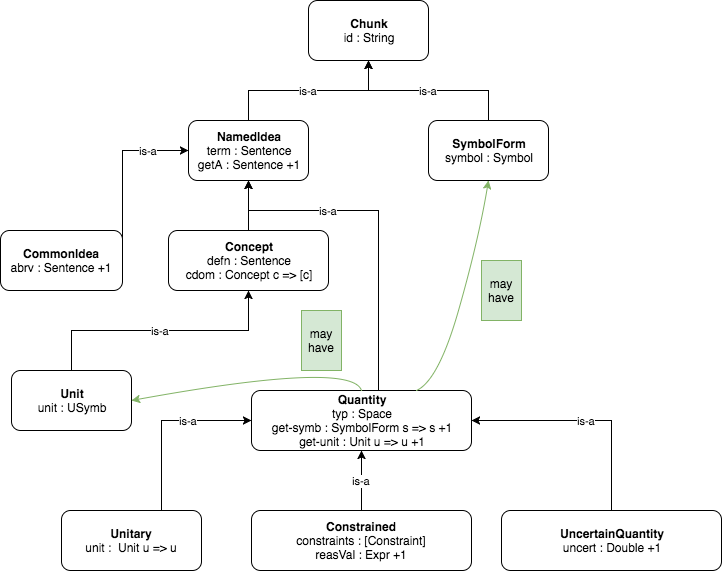
\includegraphics[width=0.5\textwidth]{figures/class_hierarchy.png}
	\caption{Drasil chunk hierarchy}
	\label{hierarchy}
\end{figure}

We can think of chunks as our building blocks of knowledge; they are the 
ingredients to be used in our \textit{Recipes}. Our language of recipes is a 
Domain-Specific Language (DSL) embedded in Haskell which is used to define what 
we would like to generate, and in what order. A small snippet of recipe 
language code for our Software Requirements Specification (SRS) can be seen in 
Figure~\ref{recipeLang}. This code is used to generate the \textit{Reference 
Materials} section of our SRS, which contains an introduction followed by the 
table of units, table of symbols, and table of abbreviations and acronyms 
subsections.

\begin{figure}
\begin{lstlisting}[language=Haskell, frame=single, showstringspaces=false, 
basicstyle=\small]
mkSRS :: DocDesc 
mkSRS = [RefSec (RefProg intro 
	[TUnits, 
	tsymb [TSPurpose, SymbOrder], 
	TAandA])]
        ...
\end{lstlisting}
\caption{The reference material section for an SRS written in Drasil's Document 
Language}
\label{recipeLang}
\end{figure}

The document generation language is highly abstracted, but allows for a fairly 
high degree of customization. Drasil also contains a code-generation language 
integrating GOOL~\cite{GOOL} -- a Generic Object-Oriented Language -- which can 
generate code in a number of different target languages including Python, Lua, 
and C++. We will discuss code generation in more depth later on.

Finally, there is the knowledge-base for Drasil (located in Data.Drasil). We 
are creating a database of reusable scientific knowledge that can be applied 
across a number of different applications across multiple domains. As the 
Drasil framework grows, we hope to continue to expand this database into an 
ontology of scientific information for a number of disciplines. See 
Figure~\ref{ontology} for an example of some of the domains in which we have 
started to capture knowledge.

\begin{figure}
	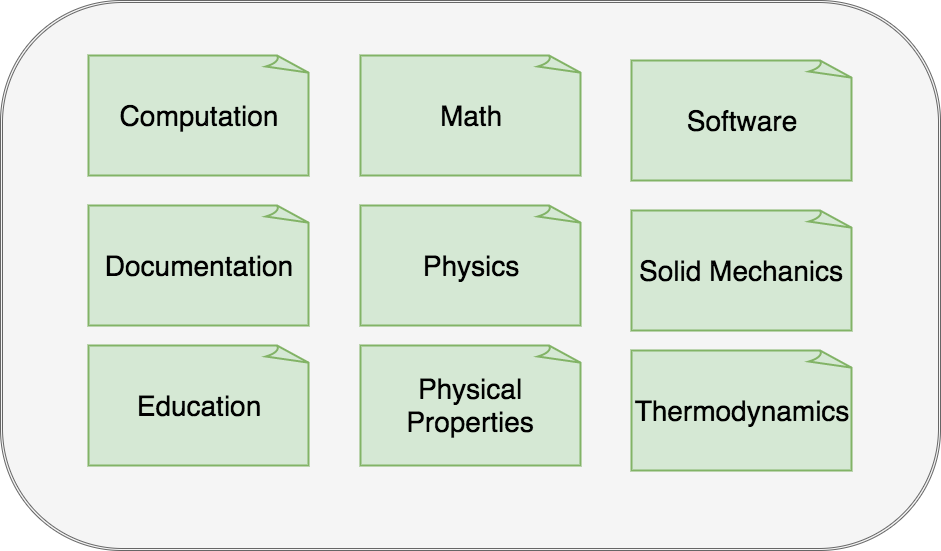
\includegraphics[width=.5\textwidth]{figures/ontology.png}
	\caption{Data.Drasil knowledge domains}
	\label{ontology}
\end{figure}

\section{Development Process for Drasil} \label{SecDevProcess}

Drasil is being developed using a practical, example-driven process. There are 
currently five different examples being developed concurrently within (and 
driving the development of) Drasil:

\begin{itemize}
\item Chipmunk2D Game Engine
\item Solar Water Heating System Incorporating Phase Change Material (PCM)
\item Solar Water Heating System (No PCM)
\item Slope Stability Analysis
\item Glass Breakage Analysis
\end{itemize}
These examples overlap with those found in~\cite{SmithJegatheesanAndKelly2016}.

Our practical design approach allows us the flexibility to prototype without 
over-designing. As a new feature becomes necessary to continue the 
implementation of a given example, only then do we design, test, implement, and 
re-test it. We occasionally implement features we may need in the future, but 
only in those instances when it is obvious that we are taking the right 
approach.

The current incarnation of the Drasil framework can be found on GitHub at 
\href{https://github.com/JacquesCarette/literate-scientific-software}
{https://github.com/JacquesCarette/literate-scientific-software}. We utilize 
peer-review of code throughout development to correct missteps early on, and 
keep an up-to-date issue tracker for any bugs, feature requests, or other 
``to-do" tasks.

%%TODO: Talk about
- refactoring - finding patterns
- knowledge extraction
- reduction of duplication


\section{GlassBR Example} \label{SecGlassBR}

- introduce example from Civil Engineering - say what the inputs are to GlassBR
and what it calculates
- bottom up approach to presentation - start with chunks, build up to SRS, traceability

- start with data definition for Jtol generated by Drasil

\begin{figure}
\begin{center}
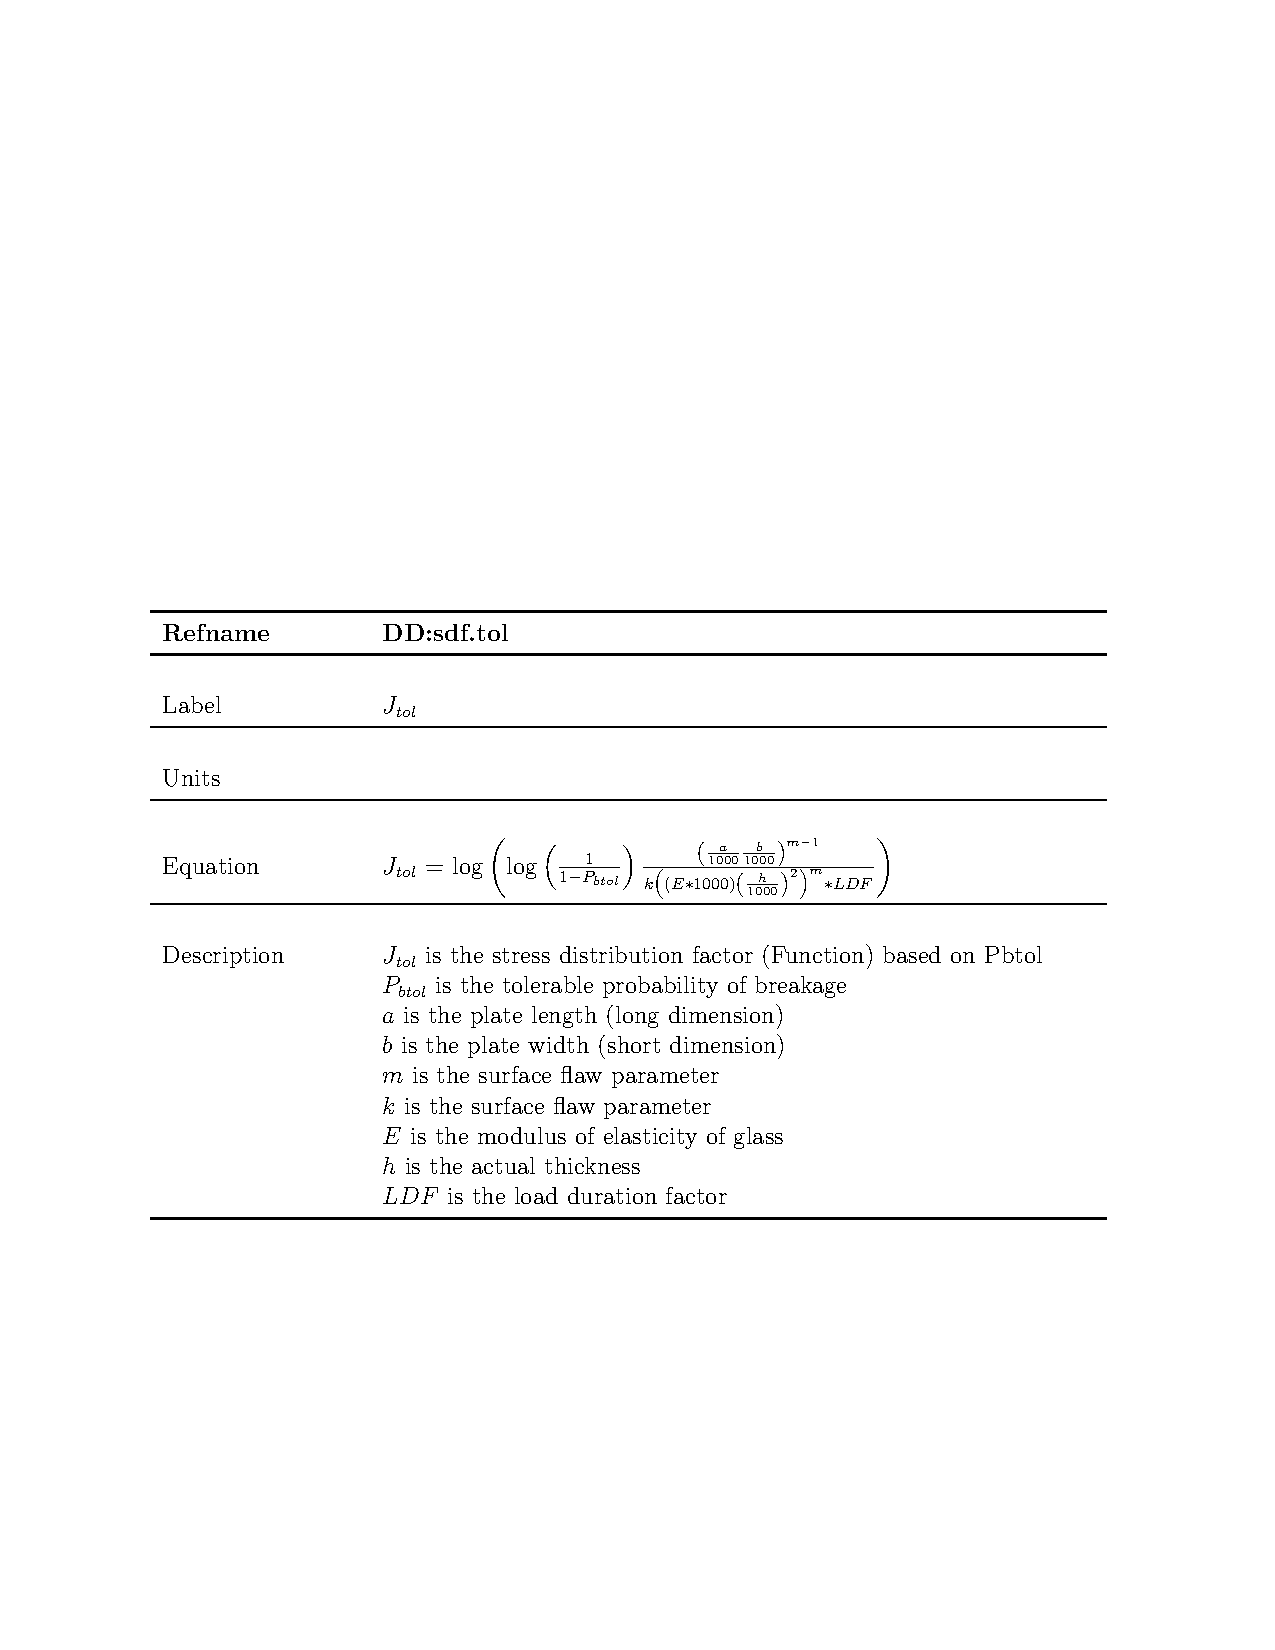
\includegraphics[width=0.45\textwidth]{./figures/Jtol_pdf.pdf}
\end{center}
\caption{$J_{\mbox{tol}}$ from GlassBR Requirements}
\label{Fig_Jtolpdf}
\end{figure}

- figure comes from tex generated by Drasil.  Can also generate html.  This
figure is part of the documentation of the requirements.  Eventually need code
to calculate Jtol.  Can generate code like in the next figure. \wss{this needs
  to be fit into one column}

\begin{figure*}
\begin{lstlisting}[language=python, frame=single, showstringspaces=false, 
basicstyle=\small]
def calc_j_tol(inparams):
    j_tol = math.log((math.log(1.0/(1.0 - inparams.pbtol))) * ((((inparams.a / 1000.0) * 
        (inparams.b / 1000.0)) ** (inparams.m - 1.0)) / ((inparams.k * (((inparams.E * 1000.0) * 
        ((inparams.h / 1000.0) ** 2.0)) ** inparams.m)) * inparams.ldf))) 
    return j_tol
\end{lstlisting}
\caption{Python code to Calculate $J_{\mbox{tol}}$}
\label{Fig_JtolPython}
\end{figure*}

- can also generate Java, Lua, etc.

- next show the source file in Drasil.  \wss{need to fit in one column}

\begin{figure*}
\begin{lstlisting}[language=Haskell, frame=single, showstringspaces=false, 
basicstyle=\small] 
stressDistFac = makeVC "stressDistFac" (nounPhraseSP $ "stress distribution" ++ " factor (Function)") cJ

sdf_tol = makeVC "sdf_tol" (nounPhraseSP $ "stress distribution" ++ " factor (Function) based on Pbtol") 
  (sub (stressDistFac ^. symbol) (Atomic "tol"))

tolStrDisFac_eq :: Expr
tolStrDisFac_eq = log (log ((1) / ((1) - (C pb_tol))) * ((Grouping (((C plate_len) / (1000)) * 
  ((C plate_width) / (1000)))) :^ ((C sflawParamM) - (1)) / ((C sflawParamK) * 
  (Grouping (Grouping ((C mod_elas) * (1000)) * (square (Grouping ((C act_thick) / (1000)))))) :^ 
  (C sflawParamM) * (C loadDF))))

tolStrDisFac :: QDefinition
tolStrDisFac = mkDataDef sdf_tol tolStrDisFac_eq
\end{lstlisting}
\caption{Drasil (Haskell) code for $J_{\mbox{tol}}$ Knowledge}
\label{Fig_JtolDrasil}
\end{figure*}

Now notice a mistake in code - shouldn't divide by 1000 - redo - fixes the
mistake everywhere

\begin{figure*}
\begin{lstlisting}[language=Haskell, frame=single, showstringspaces=false, 
basicstyle=\small]
tolStrDisFac_eq :: Expr
tolStrDisFac_eq = log (log ((1) / ((1) - (C pb_tol))) * ((Grouping ((C plate_len) * (C plate_width))) :^
  ((C sflawParamM) - (1)) / ((C sflawParamK) * (Grouping ((C mod_elas) * (square (C act_thick)))) :^ 
  (C sflawParamM) * (C loadDF))))
\end{lstlisting}
\caption{Modified Drasil (Haskell) code for $J_{\mbox{tol}}$}
\label{Fig_JtolDrasil_fix}
\end{figure*}

All of the knowledge on GlassBR can be put together to generate the software
requirements specification.  Can point to a figure showing the table of contents
for the SRS.  Explain that it can be generated in tex (pdf) or html.

\begin{figure}[htpb]
\begin{center}
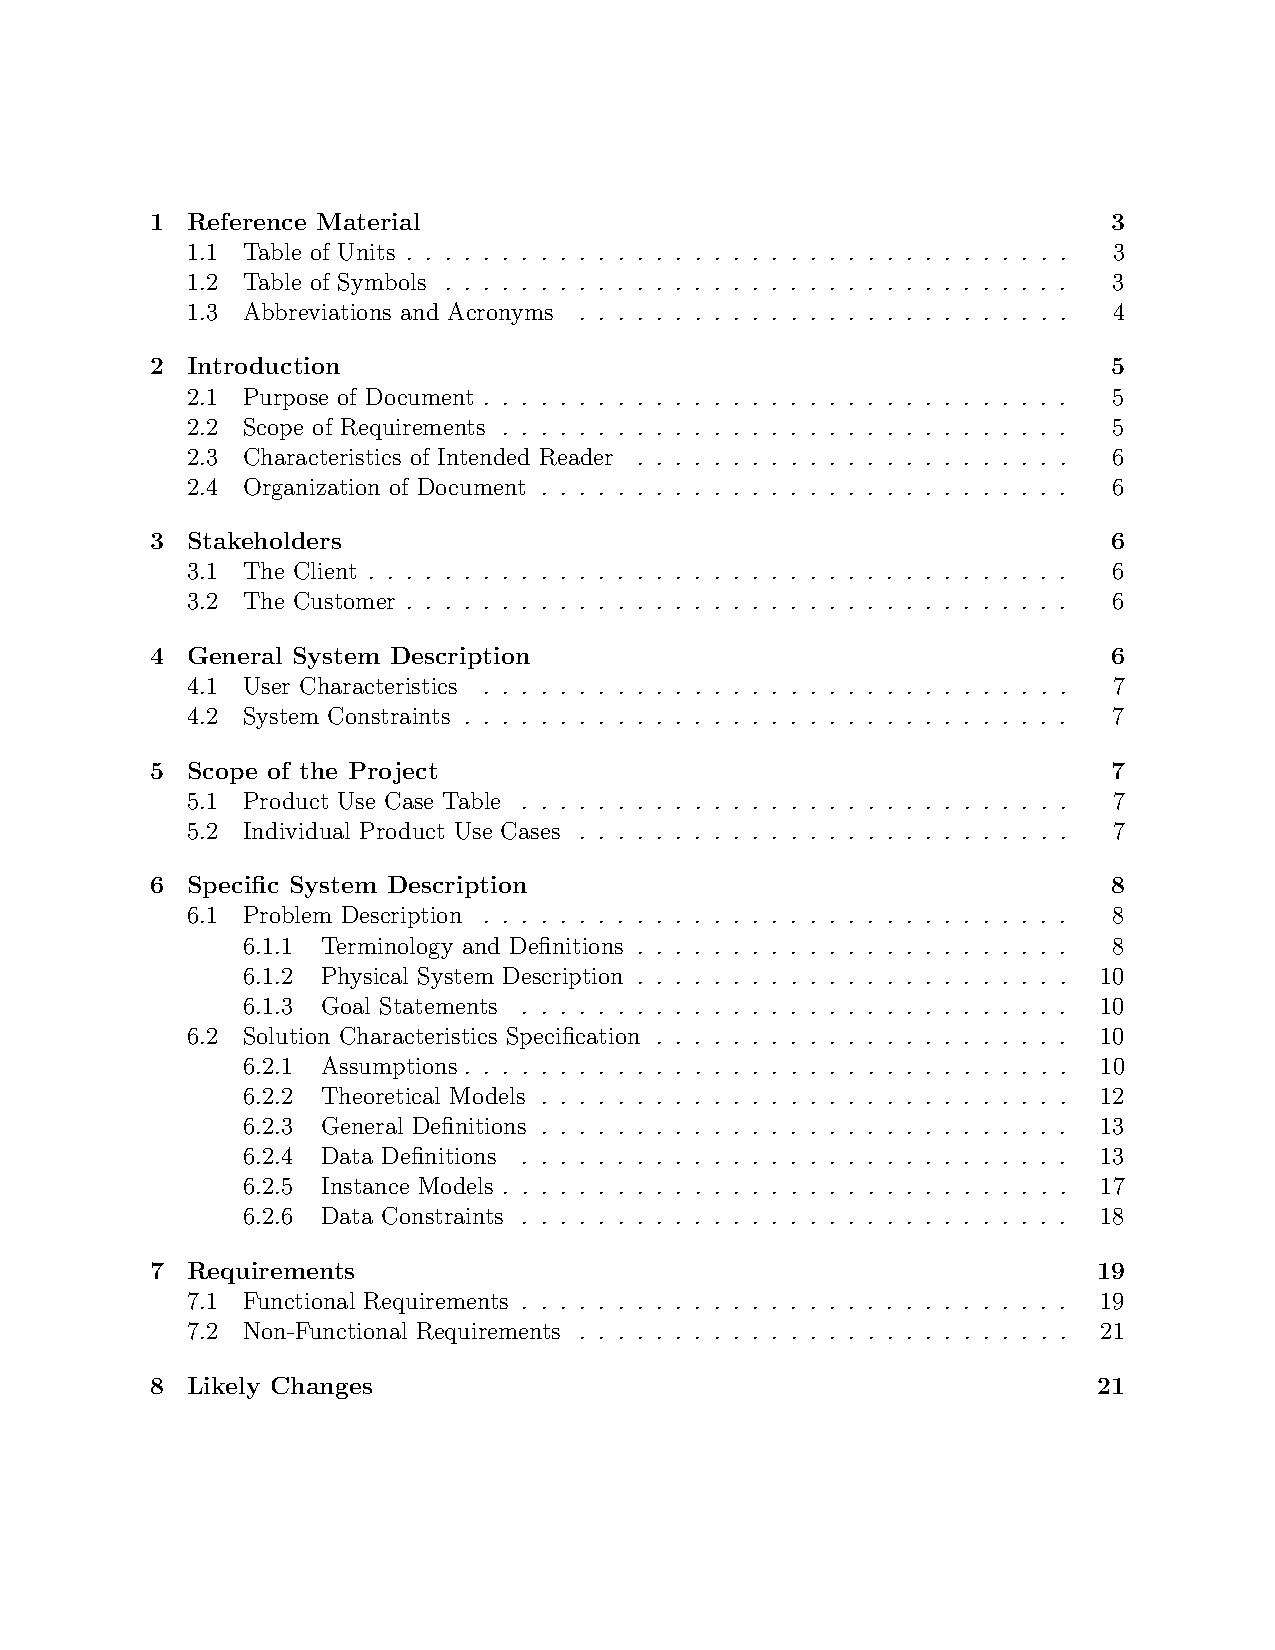
\includegraphics[scale=0.45]{./figures/TofC.pdf}
\end{center}
\caption{Table of Contents for Generated SRS for GlassBR}
\label{Fig_JtolDrasil}
\end{figure}

Part of SRS is automatically generated traceability information between
definitions, assumptions, theories and instanced models.

\begin{figure}[htpb]
\begin{center}
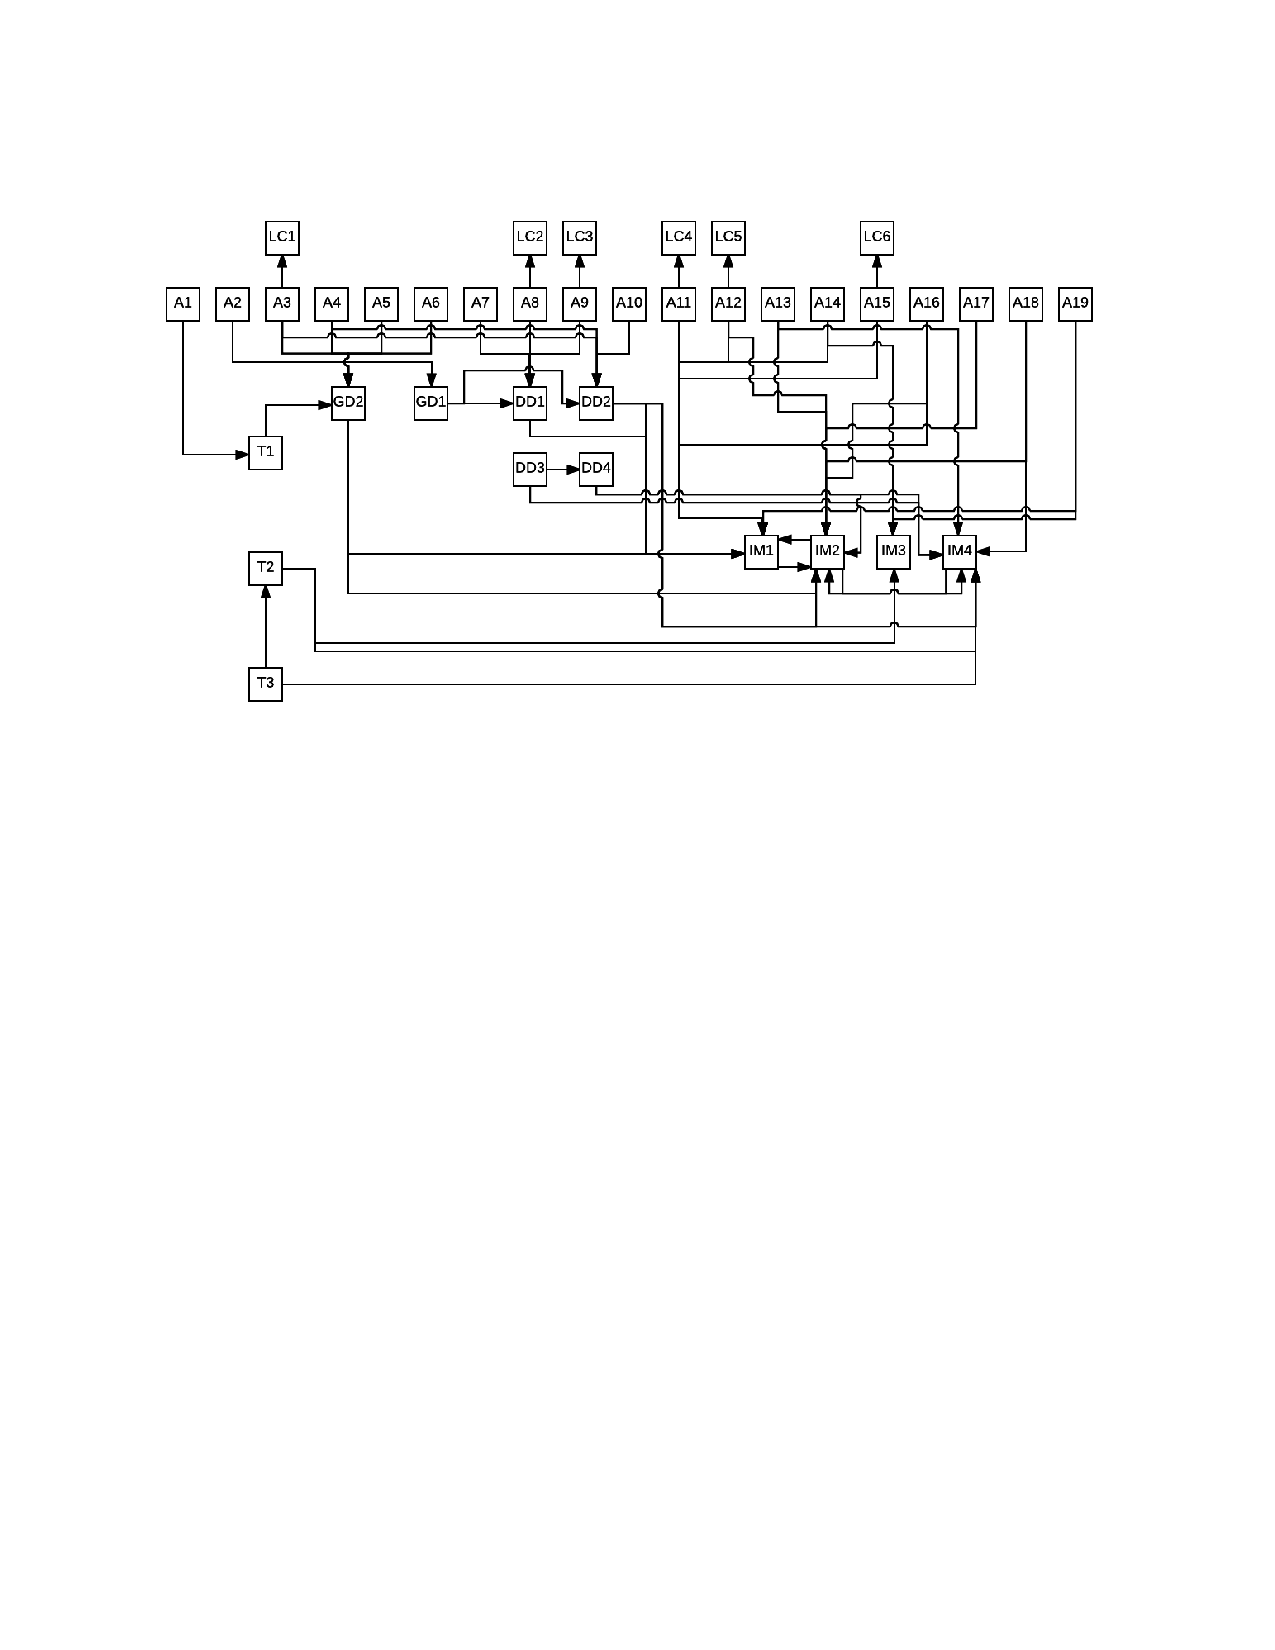
\includegraphics[scale=0.45]{./figures/TraceGraph.pdf}
\end{center}
\caption{Traceability Graph}
\label{Fig_JtolDrasil}
\end{figure}

\section{Quality Improvements} \label{SecQuality}

\subsection{Certifiability}

\begin{table} 
\centering
\caption{Constraints on quantities Used To Verify Inputs}
\begin{tabular}{c c r c } 
\toprule
\textbf{Var} & \textbf{Constraints} & \textbf{Typical Value} & \textbf{Uncertainty}\\ \midrule
$L$ & $L > 0$ & 1.5 m & 10\% \\ 
$\rho_P$ & $\rho_P > 0$	& 1007 kg/m$^3$	& 10\% \\
\bottomrule
\end{tabular}
\label{tab:pcm}
\end{table}

\begin{equation*}
E_W = \int_{0}^{t} h_C A_C (T_C - T_W(t)) dt - \int_{0}^{t} h_P A_P (T_W(t) - T_P(t)) dt
\end{equation*}

\begin{itemize}
\item \emph{If wrong, wrong everywhere}
\item Sanity checks captured and reused
\item Generate guards against invalid input
\item Generate test cases
\item Generate view suitable for inspection
\item Traceability for verification of change
\end{itemize}

\subsection{Reusability}

\begin{itemize}
\item De-embed knowledge
\item Reuse throughout document
\begin{itemize}
\item Units
\item Symbols
\item Descriptions
\item Traceability information
\end{itemize}
\item Reuse between documents
\begin{itemize}
\item SRS
\item MIS
\item Code
\item Test cases
\end{itemize}
\item Reuse between projects
\begin{itemize}
\item Knowledge reuse
\item A family of related models, or reuse of pieces
\item Conservation of thermal energy
\item Interpolation
\item Etc.
\end{itemize}
\end{itemize}

\subsection{Reproducibility}

\begin{itemize}
\item Usual emphasis is on reproducing code execution
\item However, \cite{IonescuAndJansson2013} show reproducibility challenges due to
undocumented:
\begin{itemize}
\item Assumptions
\item Modifications
\item Hacks
\end{itemize}
\item Shouldn't it be easier to independently replicate the work of others?
\item Require theory, assumptions, equations, etc.
\item Drasil can potentially check for completeness and consistency
\end{itemize}

\section{Future Work} \label{SecFuture}

\section{Concluding Remarks}

\section{Acknowledgements}

The assistance of McMaster University's Dr.\ Manuel Campidelli, Dr.\ Wael and
Dr.\ Michael Tait with the GlassBR example is greatly appreciated.

\bibliographystyle{ACM-Reference-Format}
\bibliography{SzymczakEtAl2017} 

\end{document}